% Preamble
\documentclass[12pt,a4paper]{article}
\usepackage{enumerate} 	
\usepackage{setspace}						
\usepackage{authblk}	
\usepackage{graphicx} 	
%\usepackage[nomarkers, nolists]{endfloat} 
\usepackage{pdflscape}	
\usepackage{mathtools}	
\usepackage[osf]{mathpazo} 
\usepackage{lineno} 	
\usepackage{hyperref}
\usepackage[round]{natbib} 
\usepackage{setspace}
\usepackage{longtable}
\usepackage{fancyhdr}

\setcounter{secnumdepth}{0} 
%\raggedright 			
%\pagenumbering{arabic}	
\pagenumbering{gobble}

\pagestyle{fancy}
\rhead{\textit{Guillerme \& Cooper 2018}}
\lhead{\textit{Supporting Information: S2}}
\renewcommand{\headrulewidth}{0pt}
\renewcommand{\footrulewidth}{0pt}
\setlength{\headsep}{0.3in}

\renewcommand{\thetable}{A\arabic{table}}
\renewcommand{\thefigure}{A\arabic{figure}}

% First order headings upper case bold
\usepackage{titlesec}
\titleformat*{\section}{\small\bfseries\uppercase}

% Second order headings normal case italics
\titleformat*{\subsection}{\small\itshape}

% Third order, italics, paragraph style
\titleformat*{\paragraph}{\small\itshape}

\begin{document}

\par{\centering{\Large \bf Supporting Information from ``Time for a rethink: time sub-sampling methods in disparity-through-time analyses''\par}}

\setlength{\parindent}{1cm}

\section{Appendix S2: Additional figures}

% Reset table and figure counters to 1
\setcounter{figure}{0}  
\setcounter{table}{0}  

% DTT figures
  \begin{figure}[!htbp]
    \centering
    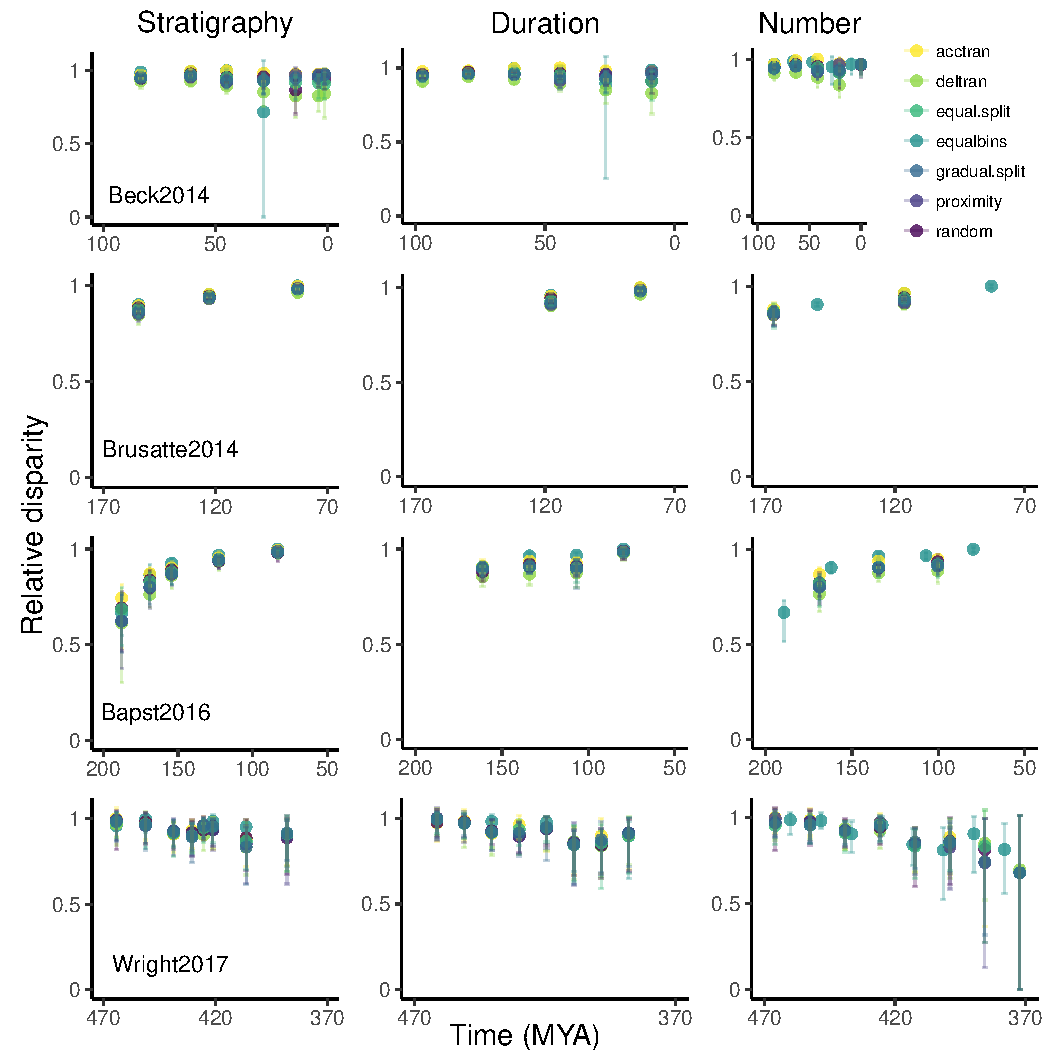
\includegraphics[width=1\linewidth, height=1\textheight, keepaspectratio]{figures/fig-dtt-epoch-appendix-revision.pdf}
    \caption[Relative disparity through time for four example datasets.]
    {Relative disparity-through-time for stratigraphic epochs. 
    Median bootstrapped disparities were calculated using time binning and time-slicing approaches. 
    Relative disparities (median bootstrapped disparity divided by the maximum median bootstrapped disparity for a dataset and analysis method) are presented so they can be compared across datasets/methods. 
    Stratigraphy uses unequal time bins or non-equidistant time-slices, where the width of the bin, or the interval between slices, is equivalent to stratigraphic epochs. 
    Duration uses equal time bins or equidistant time-slices, where the width of the bin, or the interval between slices, is the average duration of stratigraphic epochs in the time frame of the dataset. 
    Number uses equal time bins or equidistant time-slices, where the number of bins, or the number of slices, is the average number of stratigraphic epochs in the time frame of the dataset. 
    In all cases, time bin disparities are plotted at the midpoint of the bin, and error bars represent the 95\% confidence intervals around the bootstrapped median disparity.
    The four dataset names are on the first plot for each dataset (see Table 1 for details).
    Results for stratigraphic ages are shown in Figure A2.}
    \label{figure:dtt2}
  \end{figure}  

  \begin{figure}[!htbp]
    \centering
    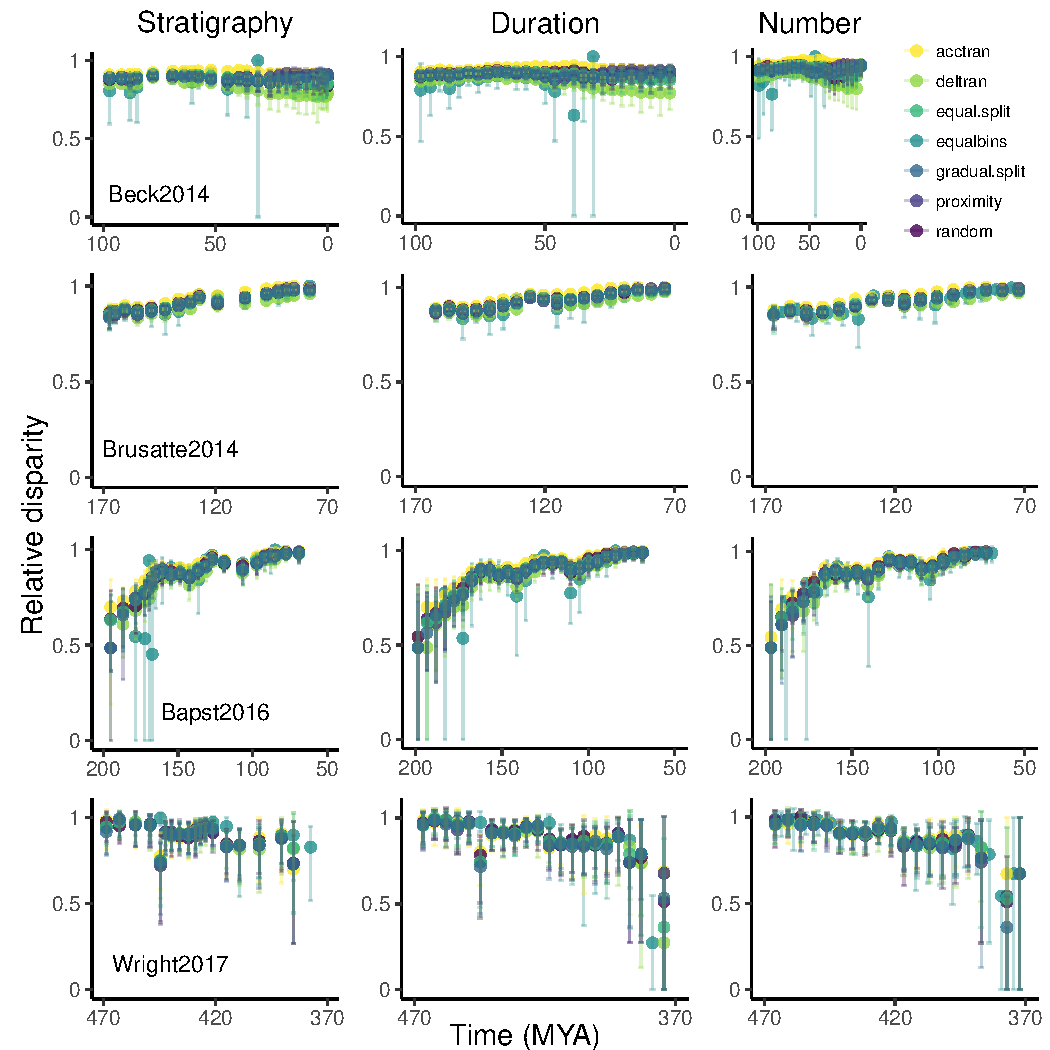
\includegraphics[width=1\linewidth, height=1\textheight, keepaspectratio]{figures/fig-dtt-age-appendix-revision.pdf}
    \caption[Relative disparity through time for four example datasets.]
    {Relative disparity-through-time for stratigraphic ages. 
    Median bootstrapped disparities were calculated using time binning and time-slicing approaches. 
    Relative disparities (median bootstrapped disparity divided by the maximum median bootstrapped disparity for a dataset and analysis method) are presented so they can be compared across datasets/methods. 
    Stratigraphy uses unequal time bins or non-equidistant time-slices, where the width of the bin, or the interval between slices, is equivalent to stratigraphic ages. 
    Duration uses equal time bins or equidistant time-slices, where the width of the bin, or the interval between slices, is the average duration of stratigraphic ages in the time frame of the dataset. 
    Number uses equal time bins or equidistant time-slices, where the number of bins, or the number of slices, is the average number of stratigraphic ages in the time frame of the dataset. 
    In all cases, time bin disparities are plotted at the midpoint of the bin, and error bars represent the 95\% confidence intervals around the bootstrapped median disparity.
    The four dataset names are on the first plot for each dataset (see Table 1 for details).
    Results for stratigraphic epochs are shown in Figure A1.}
    \label{figure:dtt3}
  \end{figure}   

% disparity peaks figures
\begin{figure}[!htbp]
    \centering
   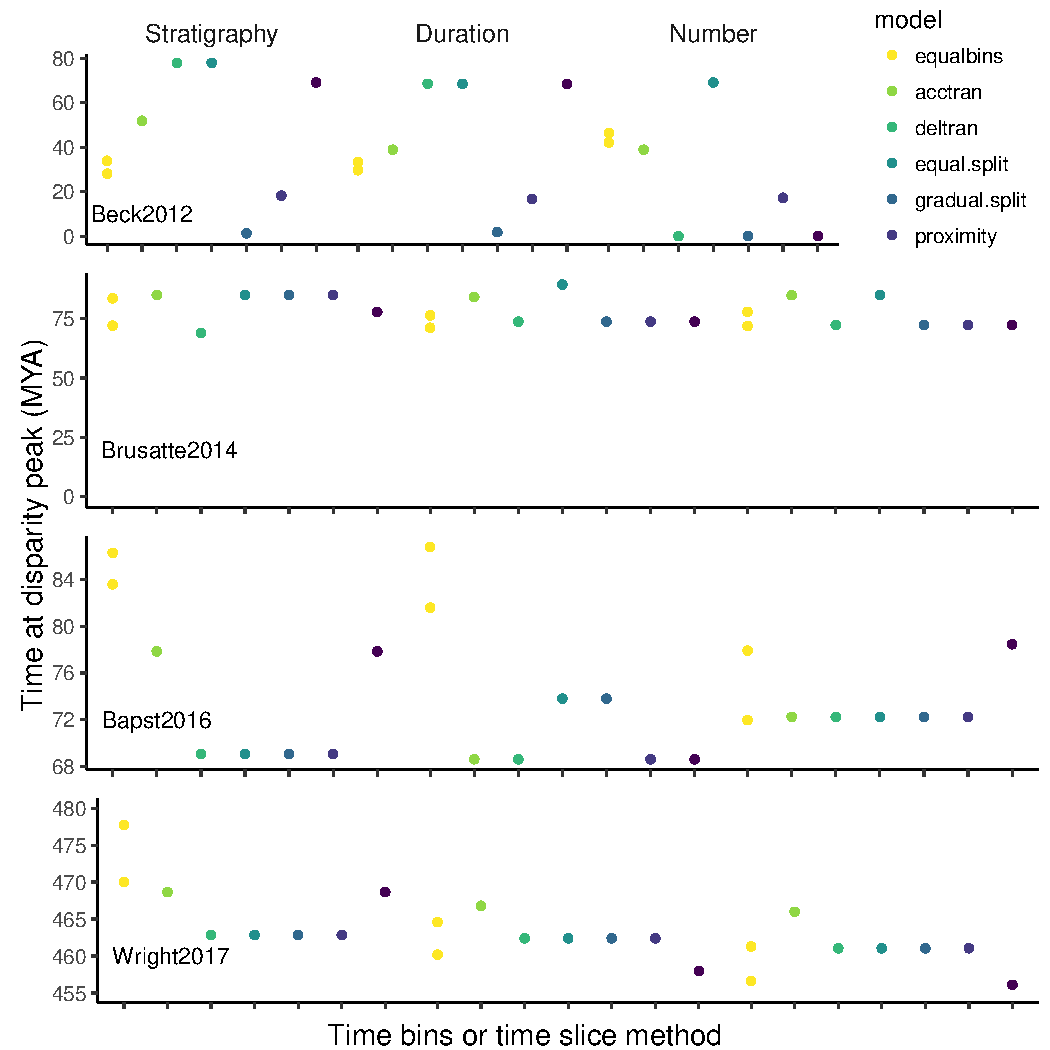
\includegraphics[width=1\linewidth, height=1\textheight, keepaspectratio]{figures/fig-peaks-epoch-appendix-revision.pdf}
    \caption[Timing of peak disparity for four example datasets.]
    {Timing of peak disparity for stratigraphic epochs.
    Median bootstrapped disparities were calculated using time binning and time-slicing approaches. 
    Stratigraphy uses unequal time bins or non-equidistant time-slices, where the width of the bin, or the interval between slices, is equivalent to stratigraphic epochs. 
    Duration uses equal time bins or equidistant time-slices, where the width of the bin, or the interval between slices, is the average duration of stratigraphic epochs in the time frame of the dataset. 
    Number uses equal time bins or equidistant time-slices, where the number of bins, or the number of slices, is the average number of stratigraphic epochs in the time frame of the dataset. 
    For time bins there are two points indicating the maximum and minimum ages of the time bin within which peak disparities appeared.
    The four dataset names are on the first plot for each dataset (see Table 1 for details).
    Results for stratigraphic ages are in Figure A4.}
    \label{figure:peak2}
  \end{figure}

\begin{figure}[!htbp]
    \centering
    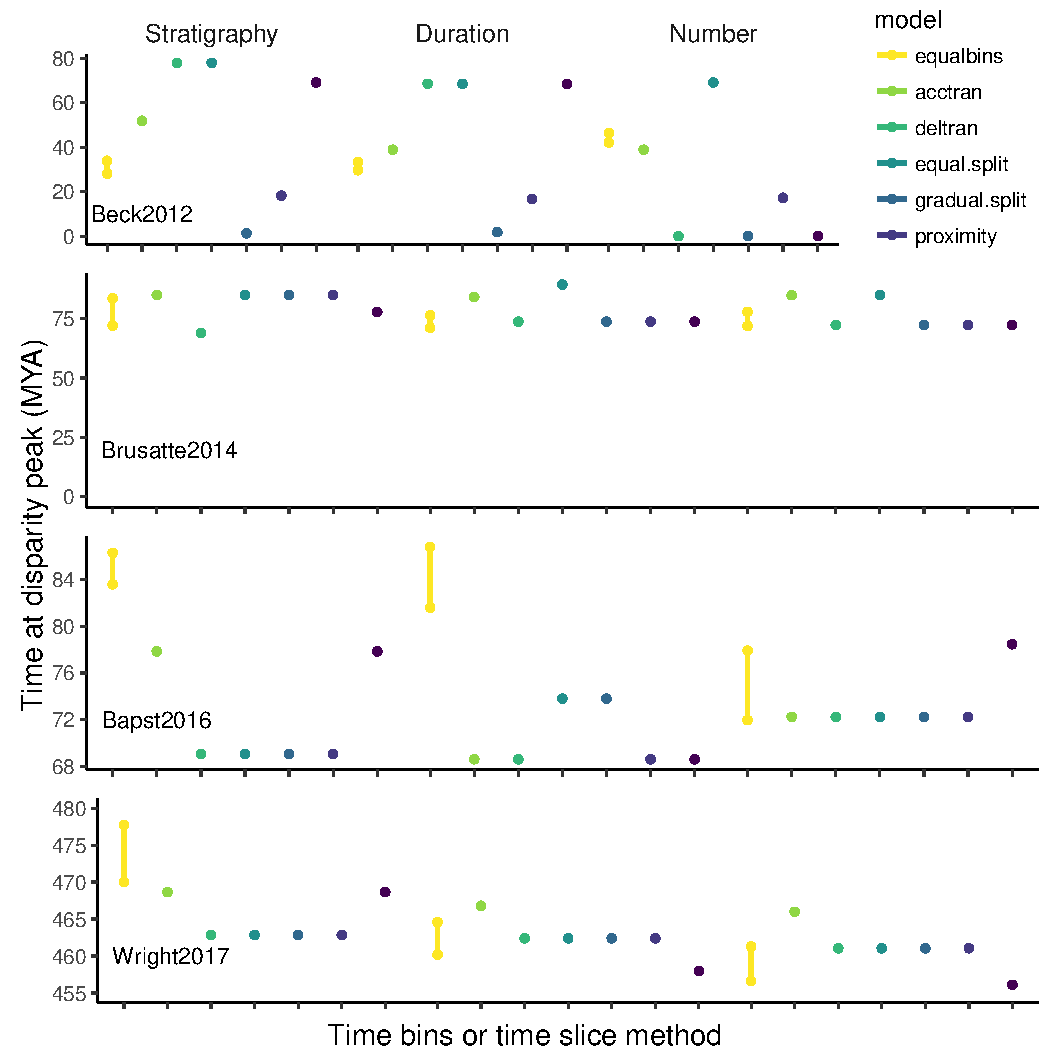
\includegraphics[width=1\linewidth, height=1\textheight, keepaspectratio]{figures/fig-peaks-age-appendix-revision.pdf}
    \caption[Timing of peak disparity for four example datasets.]
    {Timing of peak disparity for stratigraphic ages.
    Median bootstrapped disparities were calculated using time binning and time-slicing approaches. 
    Stratigraphy uses unequal time bins or non-equidistant time-slices, where the width of the bin, or the interval between slices, is equivalent to stratigraphic ages. 
    Duration uses equal time bins or equidistant time-slices, where the width of the bin, or the interval between slices, is the average duration of stratigraphic ages in the time frame of the dataset. 
    Number uses equal time bins or equidistant time-slices, where the number of bins, or the number of slices, is the average number of stratigraphic ages in the time frame of the dataset. 
    For time bins there are two points indicating the maximum and minimum ages of the time bin within which peak disparities appeared.
    The four dataset names are on the first plot for each dataset (see Table 1 for details).
    Results for stratigraphic epochs are in Figure A3.}
    \label{figure:peak3}
  \end{figure}

\end{document}